\section{Lo strato Applicativo}
\paragraph{Applicazioni} 
Le applicazioni di rete sono formate da processi distributi, su vari host. Ogni host può eseguire uno o più processi contemporaneamente. Questi processi comunicano tra loro mediante lo scambio di \textcolor{purple}{messaggi}.
\newline I livelli applicazione nei due lati della comunicazione agiscono come se esistesse un collegamento diretto su cui inviare questi messaggi.
\newline Il protocolli del livello applicativo definicono:
\begin{itemize}
    \item il tipo dei messaggi (es: di richiesta e di risposta).
    \item la sintassi dei vari tipi di messaggio (i campi del messaggio).
    \item la semantica dei campi (significato).
    \item le regole per determinare quando e come un processo invia messaggi o risponde ai messaggi.
\end{itemize}

\paragraph{Paradigmi del livello applicativo} Il modo in cui gli host devono comportarsi quando utilizzano una certa applicazione di rete dipende dal tipo di paradigma che questa applicazione utilizza:
\begin{itemize}
    \item \textbf{\textcolor{purple}{Client-Server:}} Un numero limitato di host, detti \textcolor{purple}{Server}, offrono servizi e sono sempre in attesa di richieste; al contrario, i restanti host, detti \textcolor{purple}{Client}, inviano richieste ai server per ricevere servizi.
    \item \textbf{\textcolor{purple}{Peer-to-Peer:}} Tutti gli host che utilizzano l'applicazione sono allo "pari" tra loro, tutti chiedono e ricevono servizi da tutti gli altri.
    \item \textbf{\textcolor{purple}{Misto}}
\end{itemize}

\begin{definition}[API]
    \textcolor{purple}{Application Programming Interface} Insieme di regole che un programmatore deve rispettare per utilizzare delle risorse.
\end{definition}

\paragraph{Interfaccia Socket} L'inteerfaccia socket (l'API di internet per eccellenza) e quell'interfaccia che si frappone tra il livello di applicazione e il livello di trasporto. Questa interfaccia è messa a disposizione dal sistema operativo che impolementa i 4 livelli inferiori dello stack protocollare TCP/IP.
La socket è una struttura dati formata da:
\begin{itemize}
    \item \textcolor{purple}{Indirizzo IP}: identificativo della macchina con cui vogliamo comunicare (32bit per indirizzi ipv4, 128bit per indirizzi ipv6);
    \item \textcolor{purple}{Porta}: numero a 16 bit che permette di identificare il processo sulla macchina con il quale si vuole comunicare.
\end{itemize} 

\subsection{Protocolli TCP e UDP}
Nel livello di trasporto della pila di protocolli TCP/IP i due protocolli principali sono:
\begin{itemize}
    \item \textbf{\textcolor{purple}{TCP:}} (Transmission Control Protocol) Protocollo connection-oriented, richiede una fase di setup tra client e server, che garantisce un trasporto affidabile dei dati. Fornisce inoltre meccaniscmi di controllo del flusso (il mittente non inonda il destinatario di dati) e della congestione (il mittente viene "rallentato" in caso di congestione della rete).
    \item \textbf{\textcolor{purple}{UDP:}} (User Datagram Protocol) Protocollo connection-less, non necessità di una fase di setup. Non garantisce trasporto affidabile e non presenta controlli di alcun tipo su flusso e congestione.
\end{itemize}
NB: entrambi \underline{non} forniscono garanzie di timing e banda minima.
\newline
\newline La scelta del protocollo da utilizzare dipende dalle esigenze dell'applicazione:
\begin{itemize}
    \item \textcolor{purple}{Throughput}: quanto è importante avere un certo livello di throughput per l'applicazione?
    \item \textcolor{purple}{Perdita dei dati}: il 100$\%$ dei dati trasferiti devono necessariamente arrivare a destinazione?
    \item \textcolor{purple}{Sensibilità ai ritardi}: l'applicazione è di tipo real-time?
\end{itemize}

\subsection{URI, URL E URN}
\paragraph{URI} Uniform Resource Identifier, è una forma generale per identificare una risorsa presente in rete:
\begin{itemize}
    \item \textcolor{purple}{Uniform}: uniformità della sintassi dell’identificatore, anche con meccanismi diversi di accesso;
    \item \textcolor{purple}{Resource}: qualsiasi cosa abbia un'identità (documento, servizio, immagine...);
    \item \textcolor{purple}{Identifier}: informazioni che permettono di distinguere un oggetto dagli altri.
\end{itemize} 
Esistono due principali tipologie di URI:
\begin{itemize}
    \item \textbf{\textcolor{purple}{URL:}} (Uniform Resource Locator) sottoinsieme di URI che identifica  le risorse attraverso il loro meccanismo di accesso.
    \item \textbf{\textcolor{purple}{URN:}} (Uniform Resource Name) sottoinsieme di URI che devono rimanere globalmente unici e persistenti anche quando la risorsa cessa di esistere e diventa non disponibile.
\end{itemize}

\paragraph{URL} Schema di una URL:
\newline $<$scheme$>$://$<$user$>$:$<$password$>$@$<$host$>$:$<$port$>$/$<$path$>$
\begin{itemize}
    \item $<$user$>$ e $<$password$>$ opzionale, in generale deprecato;
    \item $<$scheme$>$ indica il protocollo di accesso alla risorsa;
    \item $<$host$>$ nome di dominio di un host o indirizzo ip (in notazione decimale puntata);
    \item $<$port$>$ numero di porta del server;
    \item $<$path$>$ contiene dati specifici per l’host (o scheme) e identifica la risorsa nel contesto di quello schema e host.
\end{itemize}
A loro volta le URL possono essere di due tipologie differenti:
\begin{itemize}
    \item \textcolor{purple}{URL assoluta:} identifica una risorsa indipendentemente dal contesto in cui è usata;
    \item \textcolor{purple}{URL relativa:} informazioni per identificare una risorsa in relazione ad un’altra URL (è priva dello schema e della authority).
\end{itemize}
Le URL relative non vengono utilizzate in rete, ma vengono interpretate dal browser in relazione al documento di partenza.

\subsection{HTTP}
\paragraph{HyperText Transfer Protocol} Protocollo di tipo richiesta/risposta nel quale un client inizia la connessione, inviando al server una \textcolor{purple}{request}, e ricevendo da esso una \textcolor{purple}{response}. 
HTTP viene detto \textcolor{purple}{stateless} inquanto ogni coppia richiesta/risposta è indipendente da tutte le altre. 
Per funzionare utilizza il protocollo di trasporto TCP con il quale viene instaurata una connessione tra client e server.

\begin{definition}[Connessione]
    Un circuito logico, al livello di trasporto, stabilito tra due programmi applicativi per comunicare tra loro.    
\end{definition}
\begin{definition}[Connessione non persistente, da RFC 1945]
    Viene stabilita unaconnessione TCP separata per recuperare ciascuna URL.
\end{definition}
\begin{definition}[Connessione persistente, da RFC 2616]
    Se non diversamente indicato, il client può assumere che il server manterrà una connessione persistente.
    \begin{itemize}
        \item Lo standard specifica un meccanismo con cui client e server possono indicare la chiusura della connessione TCP (Connection header field);
        \item Dopo la chiusura, il client non deve più inviare richieste su quella connessione.
    \end{itemize}
\end{definition}

\newblock

\begin{figure}
    \centering
    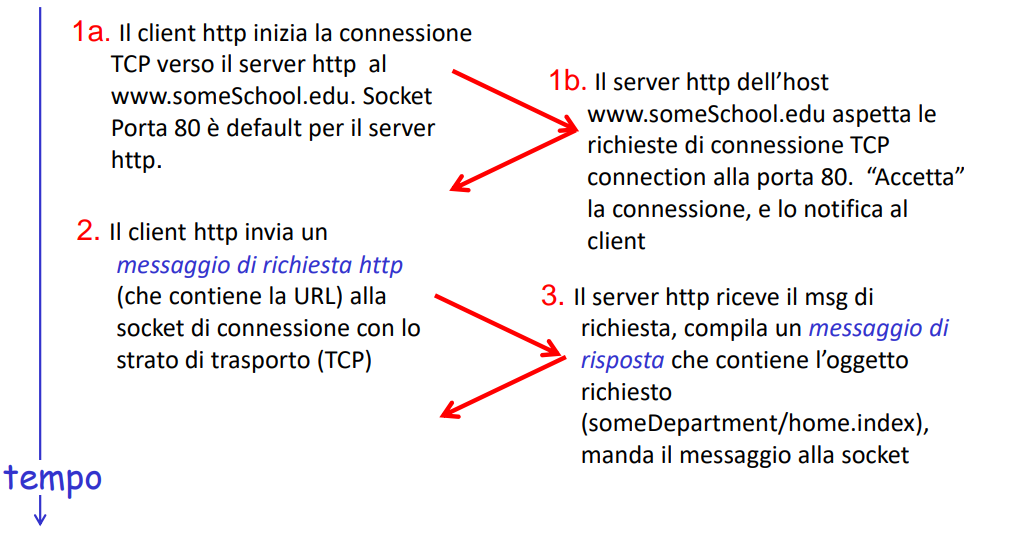
\includegraphics[scale=0.35]{Immagini/Esempio_richiesta_HTTP.png}
    \caption{Esempio di interazione con protocollo HTTP (1)}
\end{figure}

\begin{figure}[h]
    \centering
    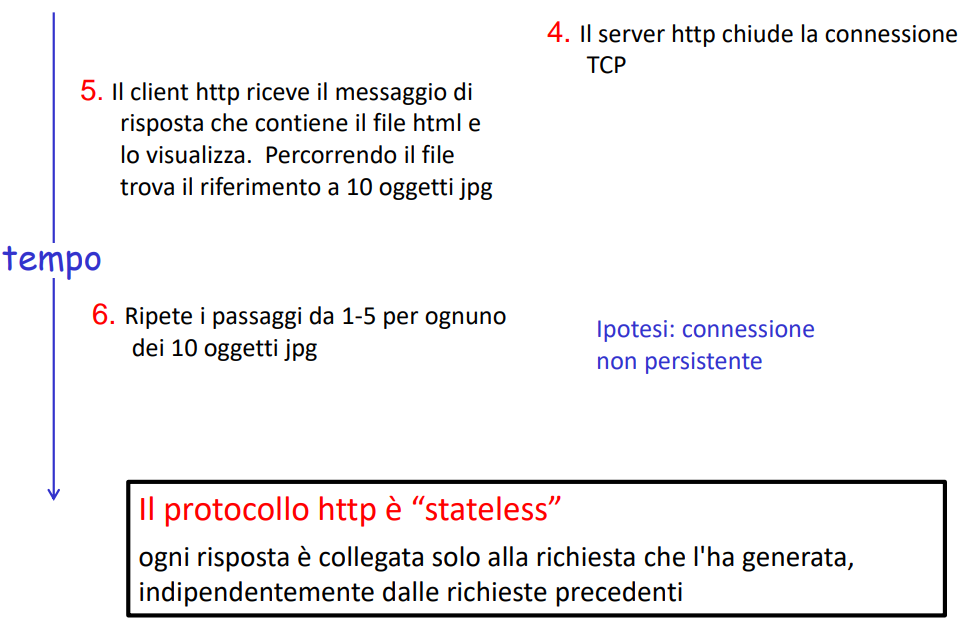
\includegraphics[scale=0.35]{Immagini/Esempio_richiesta_HTTP_2.png}
    \caption{Esempio di interazione con protocollo HTTP (2)}
\end{figure}

In caso di connessione persistente, questa non può essere utilizzata per una serie di richieste ed una corrispondente serie di risposte. Il server infatti dopo aver inviato la sua risposta rimane in attesa di altre richieste sulla connessione già aperta, fino ad una richiesta di chiusura da parte del client (che lo specifica nell'header) o in caso di attesa prolungata (time out).